%!TEX root = ../thesis.tex

\centering
  \begin{subfigure}[b]{0.98\textwidth}
    \centering
      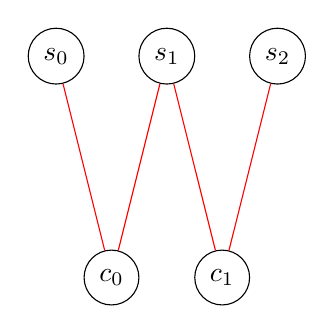
\begin{tikzpicture}
        \tikzstyle{every node}=[circle, draw]
        \foreach \i in {0, 1, 2}
        {
          \path (\i*40pt, 80pt) node (s\i) {$s_{\i}$};
        }

        \foreach \j in {0, 1}
        {
          \path (\j*40pt+20pt, 0) node (c\j) {$c_{\j}$};
        }

        \draw [red]
          (c0) -- (s0)
          (c0) -- (s1)
          (c1) -- (s1)
          (c1) -- (s2);
      \end{tikzpicture}

    \caption{\grb{} being the smallest possible red \sg{}}\label{figure:2:a}
  \end{subfigure}

  \bigskip

  \begin{subfigure}[b]{0.98\textwidth}
    \centering
      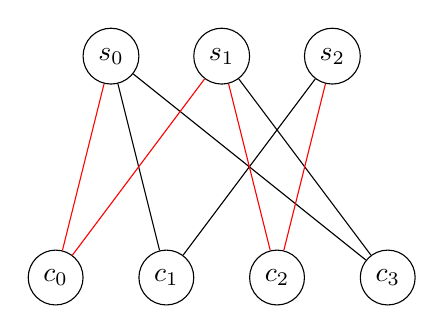
\begin{tikzpicture}
        \tikzstyle{every node}=[circle, draw]
        \foreach \i in {0, ..., 2}
        {
          \path (\i*40pt, 80pt) node (s\i) {$s_{\i}$};
        }

        \foreach \j in {0, ..., 3}
        {
          \path (\j*40pt-20pt, 0) node (c\j) {$c_{\j}$};
        }

        \draw
          (c1) -- (s0)
          (c1) -- (s2)
          (c3) -- (s0)
          (c3) -- (s1);

        \draw [red]
          (c0) -- (s0)
          (c0) -- (s1)
          (c2) -- (s1)
          (c2) -- (s2);
      \end{tikzpicture}

    \caption{\grb[1] containing a red \sg{}}\label{figure:2:b}
  \end{subfigure}

  \bigskip

  \begin{subfigure}[b]{0.98\textwidth}
    \centering
      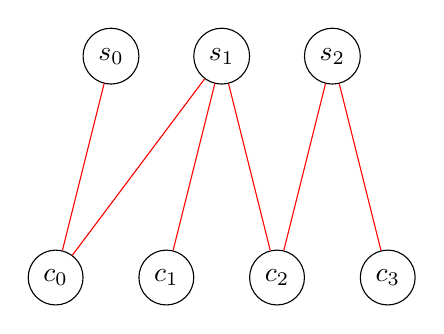
\begin{tikzpicture}
        \tikzstyle{every node}=[circle, draw]
        \foreach \i in {0, ..., 2}
        {
          \path (\i*40pt, 80pt) node (s\i) {$s_{\i}$};
        }

        \foreach \j in {0, ..., 3}
        {
          \path (\j*40pt-20pt, 0) node (c\j) {$c_{\j}$};
        }

        \draw [red]
          (c0) -- (s0)
          (c0) -- (s1)
          (c1) -- (s1)
          (c2) -- (s1)
          (c2) -- (s2)
          (c3) -- (s2);
      \end{tikzpicture}

    \caption{\grb[3] containing a red \sg{} - notice how the graph can't be emptied}\label{figure:2:c}
  \end{subfigure}
